\documentclass[10pt,aspectratio=169,serif]{beamer}

\usepackage[fontset=none, scheme=plain]{ctex}
\IfFontExistsTF{Songti SC}{%
	\setCJKmainfont{Songti SC}[AutoFakeSlant=0.2]%
	\setCJKsansfont{Songti SC}[AutoFakeSlant=0.2]%
}{%
	\setCJKmainfont{FandolSong-Regular}[Extension=.otf,BoldFont=FandolSong-Bold,AutoFakeSlant=0.2]%
	\setCJKsansfont{FandolSong-Regular}[Extension=.otf,BoldFont=FandolSong-Bold]%
}
\usepackage{amsmath,amssymb,graphicx,tikz,booktabs,multicol,calligra}
\usepackage{pgfplots}
\pgfplotsset{compat=1.18}
\usepackage{tcolorbox}
\tcbuselibrary{skins}
\usepackage{XyygU}
\usepackage{caption}
\captionsetup[figure]{name=图,labelsep=period}

\usetikzlibrary{arrows.meta,positioning,calc}

% 公式间距
\setlength{\abovedisplayskip}{0pt plus 2pt minus 2pt}
\setlength{\belowdisplayskip}{0pt plus 2pt minus 2pt}

\title[5.1 任意角和弧度制练习]{5.1 任意角和弧度制（练习）}
\subtitle{任意角 \& 弧度制}
\author{}
\institute{}
\date{2026-10-16}

\begin{document}

\begin{frame}
  \titlepage
\end{frame}

% ===================== 5.1.1 任意角 练习 =====================
\begin{frame}[t]{5.1.1 练习第1题：象限角判断}
\textbf{1.}（口答）锐角是第几象限角？第一象限角一定是锐角吗？再分别就直角、钝角来回答这两个问题。
\end{frame}

\begin{frame}[t]{5.1.1 练习第1题 解答}
\begin{tcolorbox}[colback=orange!10,colframe=orange,title=\textbf{解}]
\textbf{(1) 锐角：} $0^\circ<\alpha<90^\circ$，一定是\alert{第一象限角}；第一象限角\alert{不一定}是锐角（如 $360^\circ+30^\circ=390^\circ$ 也是第一象限角）。

\vspace{0.5em}
\textbf{(2) 直角：} $\alpha=90^\circ$，终边在 $y$ 轴正半轴上，\alert{不是任何象限角}；终边在 $y$ 轴正半轴上的角都等于 $90^\circ+k\cdot 360^\circ$，它们都不是象限角。

\vspace{0.5em}
\textbf{(3) 钝角：} $90^\circ<\alpha<180^\circ$，一定是\alert{第二象限角}；第二象限角\alert{不一定}是钝角（如 $360^\circ+120^\circ=480^\circ$ 也是第二象限角）。
\end{tcolorbox}
\end{frame}

\begin{frame}[t]{5.1.1 练习第2题：星期几的周期问题}
\textbf{2.}（口答）今天是星期三，那么 $7k\ (k\in\mathbf{Z})$ 天后的那一天是星期几？$7k\ (k\in\mathbf{Z})$ 天前的那一天是星期几？100 天后的那一天是星期几？
\end{frame}

\begin{frame}[t]{5.1.1 练习第2题 解答}
\begin{tcolorbox}[colback=orange!10,colframe=orange,title=\textbf{解}]
星期以 $7$ 天为一个周期。

\vspace{0.5em}
(1) $7k$ 天后：$7k$ 是 $7$ 的整数倍，星期数不变，仍是\alert{星期三}。

\vspace{0.5em}
(2) $7k$ 天前：同理，星期数不变，仍是\alert{星期三}。

\vspace{0.5em}
(3) $100$ 天后：
\[
100 = 14\times 7 + 2,
\]
即过了 $14$ 个完整星期还多 $2$ 天，星期三往后推 $2$ 天是\alert{星期五}。
\end{tcolorbox}
\end{frame}

\begin{frame}[t]{5.1.1 练习第3题：作角并判断象限}
\textbf{3.} 已知角的顶点与直角坐标系的原点重合，始边与 $x$ 轴的非负半轴重合，作出下列各角，并指出它们是第几象限角：
\begin{enumerate}
  \item $420^\circ$；
  \item $-75^\circ$；
  \item $855^\circ$；
  \item $-510^\circ$。
\end{enumerate}
\end{frame}

\begin{frame}[t]{5.1.1 练习第3题 解答}
\begin{tcolorbox}[colback=orange!10,colframe=orange,title=\textbf{解}]
把各角化为 $0^\circ\sim 360^\circ$ 范围内终边相同的角：

\vspace{0.3em}
(1) $420^\circ = 60^\circ + 360^\circ$，与 $60^\circ$ 终边相同，是\alert{第一象限角}。

(2) $-75^\circ = -75^\circ + 0\cdot 360^\circ$，终边在第四象限，是\alert{第四象限角}。

(3) $855^\circ = 135^\circ + 2\times 360^\circ$，与 $135^\circ$ 终边相同，是\alert{第二象限角}。

(4) $-510^\circ = 210^\circ - 2\times 360^\circ$，与 $210^\circ$ 终边相同，是\alert{第三象限角}。
\end{tcolorbox}
\end{frame}

\begin{frame}[t]{5.1.1 练习第3题 终边示意图}
\begin{center}
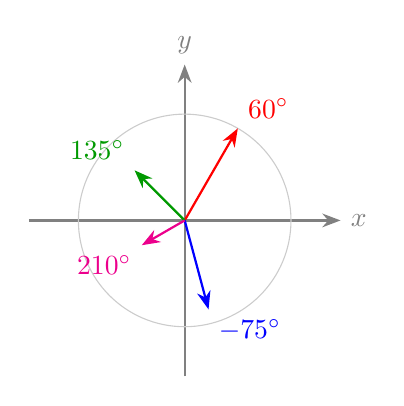
\begin{tikzpicture}[scale=0.9,>=Stealth]
\draw[->,thick,gray] (-2.2,0)--(2.2,0) node[right] {$x$};
\draw[->,thick,gray] (0,-2.2)--(0,2.2) node[above] {$y$};
\draw[gray!40] (0,0) circle (1.5);
% 60° (第一象限)
\draw[->,thick,red] (0,0)--({1.5*cos(60)},{1.5*sin(60)}) node[above right] {$60^\circ$};
% -75° (第四象限)
\draw[->,thick,blue] (0,0)--({1.3*cos(-75)},{1.3*sin(-75)}) node[below right] {$-75^\circ$};
% 135° (第二象限)
\draw[->,thick,green!60!black] (0,0)--({1.0*cos(135)},{1.0*sin(135)}) node[above left] {$135^\circ$};
% 210° (第三象限)
\draw[->,thick,magenta] (0,0)--({0.7*cos(210)},{0.7*sin(210)}) node[below left] {$210^\circ$};
\end{tikzpicture}
\end{center}
\end{frame}

\begin{frame}[t]{5.1.1 练习第4题：找终边相同的角}
\textbf{4.} 在 $0^\circ\sim 360^\circ$ 范围内，找出与下列各角终边相同的角，并指出它们是第几象限角：
\begin{enumerate}
  \item $-54^\circ 18'$；
  \item $395^\circ 8'$；
  \item $-1190^\circ 30'$。
\end{enumerate}
\end{frame}

\begin{frame}[t]{5.1.1 练习第4题 解答}
\begin{tcolorbox}[colback=orange!10,colframe=orange,title=\textbf{解}]
(1) $-54^\circ 18' + 360^\circ = 305^\circ 42'$，终边在第四象限，是\alert{第四象限角}。

\vspace{0.5em}
(2) $395^\circ 8' - 360^\circ = 35^\circ 8'$，终边在第一象限，是\alert{第一象限角}。

\vspace{0.5em}
(3) $-1190^\circ 30' + 4\times 360^\circ = -1190^\circ 30' + 1440^\circ = 249^\circ 30'$，终边在第三象限，是\alert{第三象限角}。
\end{tcolorbox}
\end{frame}

\begin{frame}[t]{5.1.1 练习第5题：终边相同的角的集合}
\textbf{5.} 写出与下列各角终边相同的角的集合，并找出集合中适合不等式 $-720^\circ\le \beta<360^\circ$ 的元素 $\beta$：
\begin{enumerate}
  \item $1303^\circ 18'$；
  \item $-225^\circ$。
\end{enumerate}
\end{frame}

\begin{frame}[t]{5.1.1 练习第5题 解答：(1)}
\begin{tcolorbox}[colback=orange!10,colframe=orange,title=\textbf{解：(1)}]
先把 $1303^\circ 18'$ 化为 $0^\circ\sim 360^\circ$ 内的角：
\[
1303^\circ 18' - 3\times 360^\circ = 1303^\circ 18' - 1080^\circ = 223^\circ 18'.
\]
终边相同的角的集合：
\[
S = \{\beta \mid \beta = 223^\circ 18' + k\cdot 360^\circ,\ k\in\mathbf{Z}\}.
\]
取 $k=-2,-1,0$：
\[
\beta = 223^\circ 18' - 720^\circ = -496^\circ 42',
\]
\[
\beta = 223^\circ 18' - 360^\circ = -136^\circ 42',
\]
\[
\beta = 223^\circ 18'.
\]
所以 $\beta\in \{-496^\circ 42',\ -136^\circ 42',\ 223^\circ 18'\}$。
\end{tcolorbox}
\end{frame}

\begin{frame}[t]{5.1.1 练习第5题 解答：(2)}
\begin{tcolorbox}[colback=orange!10,colframe=orange,title=\textbf{解：(2)}]
$-225^\circ$ 本身就在 $-360^\circ\sim 360^\circ$ 范围内。

终边相同的角的集合：
\[
S = \{\beta \mid \beta = -225^\circ + k\cdot 360^\circ,\ k\in\mathbf{Z}\}.
\]
取 $k=-1,0,1$：
\[
\beta = -225^\circ - 360^\circ = -585^\circ,
\]
\[
\beta = -225^\circ,
\]
\[
\beta = -225^\circ + 360^\circ = 135^\circ.
\]
所以 $\beta\in \{-585^\circ,\ -225^\circ,\ 135^\circ\}$。
\end{tcolorbox}
\end{frame}

% ===================== 5.1.2 弧度制 练习 =====================
\begin{frame}[t]{5.1.2 练习第1题：角度化弧度}
\textbf{1.} 把下列角度化成弧度：
\begin{enumerate}
  \item $22^\circ 30'$；
  \item $-210^\circ$；
  \item $1200^\circ$。
\end{enumerate}
\end{frame}

\begin{frame}[t]{5.1.2 练习第1题 解答}
\begin{tcolorbox}[colback=orange!10,colframe=orange,title=\textbf{解}]
换算关系：$1^\circ = \dfrac{\pi}{180}$ rad。

\vspace{0.3em}
(1) $22^\circ 30' = 22.5^\circ = \dfrac{45}{2}^\circ$，
\[
22^\circ 30' = \frac{45}{2}\times\frac{\pi}{180} = \alert{\frac{\pi}{8}}\ \text{rad}.
\]

(2) $-210^\circ = -210\times\dfrac{\pi}{180} = \alert{-\dfrac{7\pi}{6}}$ rad。

(3) $1200^\circ = 1200\times\dfrac{\pi}{180} = \alert{\dfrac{20\pi}{3}}$ rad。
\end{tcolorbox}
\end{frame}

\begin{frame}[t]{5.1.2 练习第2题：弧度化角度}
\textbf{2.} 把下列弧度化成角度：
\begin{enumerate}
  \item $\dfrac{\pi}{12}$；
  \item $-\dfrac{4\pi}{3}$；
  \item $\dfrac{3\pi}{10}$。
\end{enumerate}
\end{frame}

\begin{frame}[t]{5.1.2 练习第2题 解答}
\begin{tcolorbox}[colback=orange!10,colframe=orange,title=\textbf{解}]
换算关系：$1\ \text{rad} = \left(\dfrac{180}{\pi}\right)^\circ$，即 $\pi\ \text{rad}=180^\circ$。

\vspace{0.3em}
(1) $\dfrac{\pi}{12} = \dfrac{180^\circ}{12} = \alert{15^\circ}$。

(2) $-\dfrac{4\pi}{3} = -\dfrac{4}{3}\times 180^\circ = \alert{-240^\circ}$。

(3) $\dfrac{3\pi}{10} = \dfrac{3}{10}\times 180^\circ = \alert{54^\circ}$。
\end{tcolorbox}
\end{frame}

\begin{frame}[t]{5.1.2 练习第3题：坐标轴上的角的集合}
\textbf{3.} 用弧度表示：
\begin{enumerate}
  \item 终边在 $x$ 轴上的角的集合；
  \item 终边在 $y$ 轴上的角的集合。
\end{enumerate}
\end{frame}

\begin{frame}[t]{5.1.2 练习第3题 解答}
\begin{tcolorbox}[colback=orange!10,colframe=orange,title=\textbf{解}]
(1) 终边在 $x$ 轴上的角，在 $0\sim 2\pi$ 内有 $0$ 和 $\pi$，间隔为 $\pi$：
\[
\alert{S_x = \{\beta \mid \beta = k\pi,\ k\in\mathbf{Z}\}}.
\]

\vspace{0.5em}
(2) 终边在 $y$ 轴上的角，在 $0\sim 2\pi$ 内有 $\dfrac{\pi}{2}$ 和 $\dfrac{3\pi}{2}$，间隔为 $\pi$：
\[
\alert{S_y = \left\{\beta \mid \beta = \frac{\pi}{2} + k\pi,\ k\in\mathbf{Z}\right\}}.
\]
\end{tcolorbox}
\end{frame}

\begin{frame}[t]{5.1.2 练习第4题：角度制与弧度制下三角函数值比较}
\textbf{4.} 利用计算工具比较下列各对值的大小：
\begin{enumerate}
  \item $\cos 0.75^\circ$ 和 $\cos 0.75$；
  \item $\tan 1.2^\circ$ 和 $\tan 1.2$。
\end{enumerate}
\end{frame}

\begin{frame}[t]{5.1.2 练习第4题 解答}
\begin{tcolorbox}[colback=orange!10,colframe=orange,title=\textbf{解}]
注意：$\cos 0.75$ 中 $0.75$ 是弧度，约为 $43^\circ$。

\vspace{0.3em}
(1) $0.75^\circ$ 是很小的角，$\cos 0.75^\circ \approx 0.9999$；
而 $0.75\ \text{rad} \approx 43^\circ$，$\cos 0.75 \approx 0.7317$。
\[
\alert{\cos 0.75^\circ > \cos 0.75}.
\]

\vspace{0.5em}
(2) $1.2^\circ$ 很小，$\tan 1.2^\circ \approx 0.0209$；
而 $1.2\ \text{rad} \approx 68.8^\circ$，$\tan 1.2 \approx 2.572$。
\[
\alert{\tan 1.2^\circ < \tan 1.2}.
\]
\end{tcolorbox}
\end{frame}

\begin{frame}[t]{5.1.2 练习第5题：弧长公式}
\textbf{5.} 分别用角度制、弧度制下的弧长公式，计算半径为 $1\,\text{m}$ 的圆中，$60^\circ$ 的圆心角所对的弧的长度（可用计算工具）。
\end{frame}

\begin{frame}[t]{5.1.2 练习第5题 解答}
\begin{tcolorbox}[colback=orange!10,colframe=orange,title=\textbf{解}]
\textbf{角度制公式：} $l = \dfrac{n\pi R}{180}$，其中 $n=60$，$R=1$：
\[
l = \frac{60\cdot\pi\cdot 1}{180} = \frac{\pi}{3}\approx 1.047\ \text{m}.
\]

\vspace{0.5em}
\textbf{弧度制公式：} $l = |\alpha| R$，其中 $\alpha = 60^\circ = \dfrac{\pi}{3}$：
\[
l = \frac{\pi}{3}\times 1 = \frac{\pi}{3}\approx 1.047\ \text{m}.
\]

\vspace{0.5em}
两种公式结果一致，弧长为 $\alert{\dfrac{\pi}{3}\,\text{m}\approx 1.05\,\text{m}}$。
\end{tcolorbox}
\end{frame}

\begin{frame}[t]{5.1.2 练习第6题：求圆心角弧度数}
\textbf{6.} 已知半径为 $120\,\text{mm}$ 的圆上，有一条弧的长是 $144\,\text{mm}$，求该弧所对的圆心角（正角）的弧度数。
\end{frame}

\begin{frame}[t]{5.1.2 练习第6题 解答}
\begin{tcolorbox}[colback=orange!10,colframe=orange,title=\textbf{解}]
由弧度制下弧长公式 $l = |\alpha| R$，得
\[
|\alpha| = \frac{l}{R} = \frac{144}{120} = \alert{1.2\ \text{rad}}.
\]
因为求的是正角，所以该弧所对圆心角为 $\alert{1.2}$ 弧度。
\end{tcolorbox}
\end{frame}

\begin{frame}[c]
  \begin{center}
    {\Huge\calligra Thanks!}
  \end{center}
\end{frame}

\end{document}
